
\documentclass[runningheads,a4paper]{llncs}

\usepackage{amssymb}
%\setcounter{tocdepth}{3}
\usepackage{graphicx}
\linespread{2}
\usepackage{url}
\urldef{\mailsa}\path|{jharri1}@gmu.edu|
\newcommand{\keywords}[1]{\par\addvspace\baselineskip
\noindent\keywordname\enspace\ignorespaces#1}

%\usepackage[caption=false]{subfig}
\usepackage{wrapfig}
%\usepackage{multicol}
\usepackage{amsmath}
\usepackage{color}
\usepackage{xcolor}
\usepackage{listings}
\usepackage{subfigure}


\usepackage{caption}
\DeclareCaptionFont{white}{\color{white}}
\DeclareCaptionFormat{listing}{\colorbox{gray}{\parbox{\textwidth}{#1#2#3}}}
\captionsetup[lstlisting]{format=listing,labelfont=white,textfont=white}

\lstset{
	language=Java,
	basicstyle=\small\sffamily,
	tabsize=4,
	numbers=left
}

\renewcommand{\topfraction}{0.85}
\renewcommand{\textfraction}{0.1}
\renewcommand{\floatpagefraction}{0.75}

\providecommand{\abs}[1]{\lvert#1\rvert}

\newcommand{\doctitle}[0]{Retirement Redux: A replication of Axtell's and Epstein's Retirment Age model}

\begin{document}
\title{\doctitle}
%\shorttitle{Retirement Redux}
\author{Ernesto Carrella \\ Joseph F. Harrison}
\authorrunning{\doctitle}
\institute{George Mason University}

\toctitle{\doctitle}
\tocauthor{Authors' Instructions}
\maketitle

\section*{Abstract}
This is the Abstract
\section{Introduction}
\label{sec:intro}

We replicated Axtell's and Epstein's Retirement Age model\cite{axtell_coordination_2006}.

\section{Model Description}

The model simulates retirement decision of heterogeneous agents.
Agents differ one from the other in terms of their behavior rules, social network and death age.
Every year every agent decides whether to retire or keep working. 

There are three tipes of agents.
Random agents choose whether to retire or not by tossing a coin.
Rational agents always retire as soon as possible.
Imitators instead do what the majority of eligibles do in their social network.

The main feature of the model is the gradual emergence of retirement norms.
Although 65 is fixed to be the retirement age, the population decides to retire at that age only gradually.
This paper tries to model retirement decision without economic rationale.
Mimesis is all that matter.

\section{Replication}

\subsection{MASON}

We decided to replicate the model trough the MASON framework \cite{luke2005mason}.
This allows for the use of premade structures when programming in Java.
We did not have, nor we should have had, access to the original code in C.
Replication would be invalidated if we used anything but the original paper.

This allowed for the highlighting of both some advantages and disadvantages of Java and MASON.
These should be weighted by the added difficulty of not using NETLOGO or other ABM-specific languages.
One should also keep in mind that the original paper was also object oriented.

The greatest advantage of using Java is the ability to use premade structures.
We used an \textit{ArrayList} to store Agent's networks.
This allows us to remove deceased friends and to modify the size of the network over time.
For this very simple model, everything else would have been an overkill.

Another great advantage of Java is the proliferance of other packages we can integrate to our model.
OpenCSV was used to output formatted data.
Network packages like JUNG would have had very little added value.
Again, the simplicity of the model didn't call for any addition.

One feature of MASON is the complete separation between the graphic and the model code.
We decided to put this to a test so that each team-mate would focus on only one side of the code.
This proved not very succesful.
The model-side had to be progressively modified so that it would update the graphics-side at critical times.
This is particularly troublesome given the fact that in this model the graphical side is ancilliary.

\subsection{Object Orientation}

Intuitively, agents in this model share many similiarities.
They age, they die, they are either allowed or not to retire.
They are heterogeneous both in their endowments and their behavior.

Code-wise their different endowments are their variables, their different behavior are their class structure.
We can take advantage of Java's OO paradigm.
The UML diagram in figure~\ref{UML} describes the approach taken.
Most of the behavior is recicled from the \textit{Agent} abstract class.
Each subclass then overrides only the code pertaining retirement decision.

\begin{figure}
 \begin{center}
  \includegraphics[scale=.45]{figs/UML.png}
\caption{The class structure of the agents}
\label{UML}
 \end{center}
\end{figure}

We decided to make the super-class Agent as abstract rather than interface so that we could write common behavior together.
Classes in MASON are agents when they implement the \textit{Steppable} interface.
The Agent's step method is described in code~\ref{step}.
This allows for sub-classes to override the \textit{doIRetire} function and still use aging and death of the super-class.
{
\linespread{1}
\begin{lstlisting}[float,caption= {Agent's step class}, label={step}]
public void step(SimState arg0) {
		
		age++;

		if(age >= deathAge){
			this.die();
		}
		else if (status == Status.WORKING && age>= model.retirementAge)	
			status = doIRetire();	
	}

\end{lstlisting}
}

\subsection{Garbage Collection}

An important feature of Java is automatic garbage collection.
The programmer doesn't manually affect memory allocation. 
His responsibility is to remove any reference to the object he wants to delete.

Garbage collection proved quite a headache in our project.
All references to agents are stored in a single matrix.
We had hoped that removing these agents from the matrix would be enough to clean the memory.
It was not so.

Two components made garbage collection a major problem during development.
The first was the MASON scheduler itself.
To run an agent in MASON one needs to schedule it.
Under the hood this means holding a reference of the agent in one \textit{heap} object, preventing garbage collection.
Scheduling comes into two types: scheduling once or scheduling forever.
Because our agents had to act every year, we scheduled them forever but that made their reference permanent in the heap.

This forced us into a ``least-worst'' analysis of our design choices.
We could schedule agents once every turn by checking if they were still alive.
This would have been burdensome as we would have had to create a new steppable just to make the check every turn.
Similiarly we could have made the matrix holding agents steppable and let it activate agents directly.
But with this we would have lost many advantages of the premade \textit{Schedule} class, in particular automatic shuffling of activation order.
The third way was to try and remove agents in the scheduler manually.

Stopping an agent scheduled forever proved more troublesome than it should be.
The \textit{Schedule} class does not allow for direct removal. 
The \textit{Steppable} interface, common to all agents, does not allow for stopping.
An unrelated \textit{Stoppable} is returned when the agent is first scheduled.
What we had to do was to manually store the reference to the stoppable and pass it to the agent after it has been scheduled.
Only then the agent dies can finally stop itself.

The other garbage collection issue was with social networks.
Agents every year purge their networks of their deceased friends. 
But when they ``die'' the remaining references in the \textit{ArrayList} are automatically not removed.
This meant that some of the old social networks referenced each other even when all its agents were dead.
This prevented them from being garbage-collected.


\subsection{Visualization}

The original model by Axtell and Epstein contained a unique custom graphical user interface (GUI) that we set out to match as closely as possible. 
This required us to overcome some obstacles due to the conventions of MASON visualization. 
For instance, MASON's grid's store items in a 2D array where the first index corresponds to the $x$ coordinate of the object and the second index corresponds to the $y$ coordinate. 
Specifically, ObjectGrid2D defines the array as \lstinline!public Object[/**x*/][/**y*/] field;! This presents a challenge when we want to access a cohort in a single array since \lstinline!field[i]! gives the $i^{th}$ column of cells. In the original model, cohorts are arranged as rows.


\begin{figure}
\centering
  \subfigure[Original Paper]{
   \includegraphics[width=0.9\textwidth] {figs/orig-gui-screenshot.png}
 }
 \subfigure[MASON replication]{
   \includegraphics[width=0.9\textwidth] {figs/gui-screenshot1.png}
 }

\caption{Comparison of the original visualization with the visualization in the replication MASON model. }
\label{fig:gui-comparison}
\end{figure}


\section{Results}
Replication was only a partial success. 
In most cases we achieved relational equivalence \cite{springerlink:10.1007/BF01299065} rather than numerical identity.
In a few situations docking simply failed.

The behavior of standard cases was replicated successfully.
Figure~\ref{figure4} and figure~\ref{figure5} show side by side the retiring behavior of the system and our replication.
Every parameter was set as in the original paper.

\begin{figure}
\centering
  \subfigure[Original Paper]{
   \includegraphics[scale =.40] {figs/figure4.png}
 }
 \subfigure[MASON replication]{
   \includegraphics[scale =.13] {figs/figure4_replication.png}
 }

\caption{20\% rational agents case comparison}
\label{figure4}
\end{figure}

\begin{figure}
\centering
  \subfigure[Original Paper]{
   \includegraphics[scale =.40] {figs/figure5.png}
 }
 \subfigure[MASON replication]{
   \includegraphics[scale =.13] {figs/figure5_replication.png}
 }

\caption{5\% rational agents case comparison}
\label{figure5}
\end{figure}

We manage to replicate the fact that the less rational agents, the more it takes for society to retire.
We also managed to replicate the loss of monotonicity as rational agents decrease in numbers.
We couldn't replicate numerically the waiting period, unfortunately.
Figure~\ref{figure5}'s replication takes a fourth of the time it took the original model to let mass-retirement emerge.



\subsection{Parameter Sweep}

Parameter sweep replication was less successful than the previous chapter.
Figure~\ref{figure6} shows the difference in replicating runs by switching the proportion of agents in the population.
On one side the results are decent enough: the more the population is dominated by imitators the more it takes to retire en masse.
On the other the numbers are very different.

\begin{figure}
\centering
  \subfigure[Original Paper]{
   \includegraphics[scale =.70] {figs/figure6.png}
 }
 \subfigure[MASON replication]{
   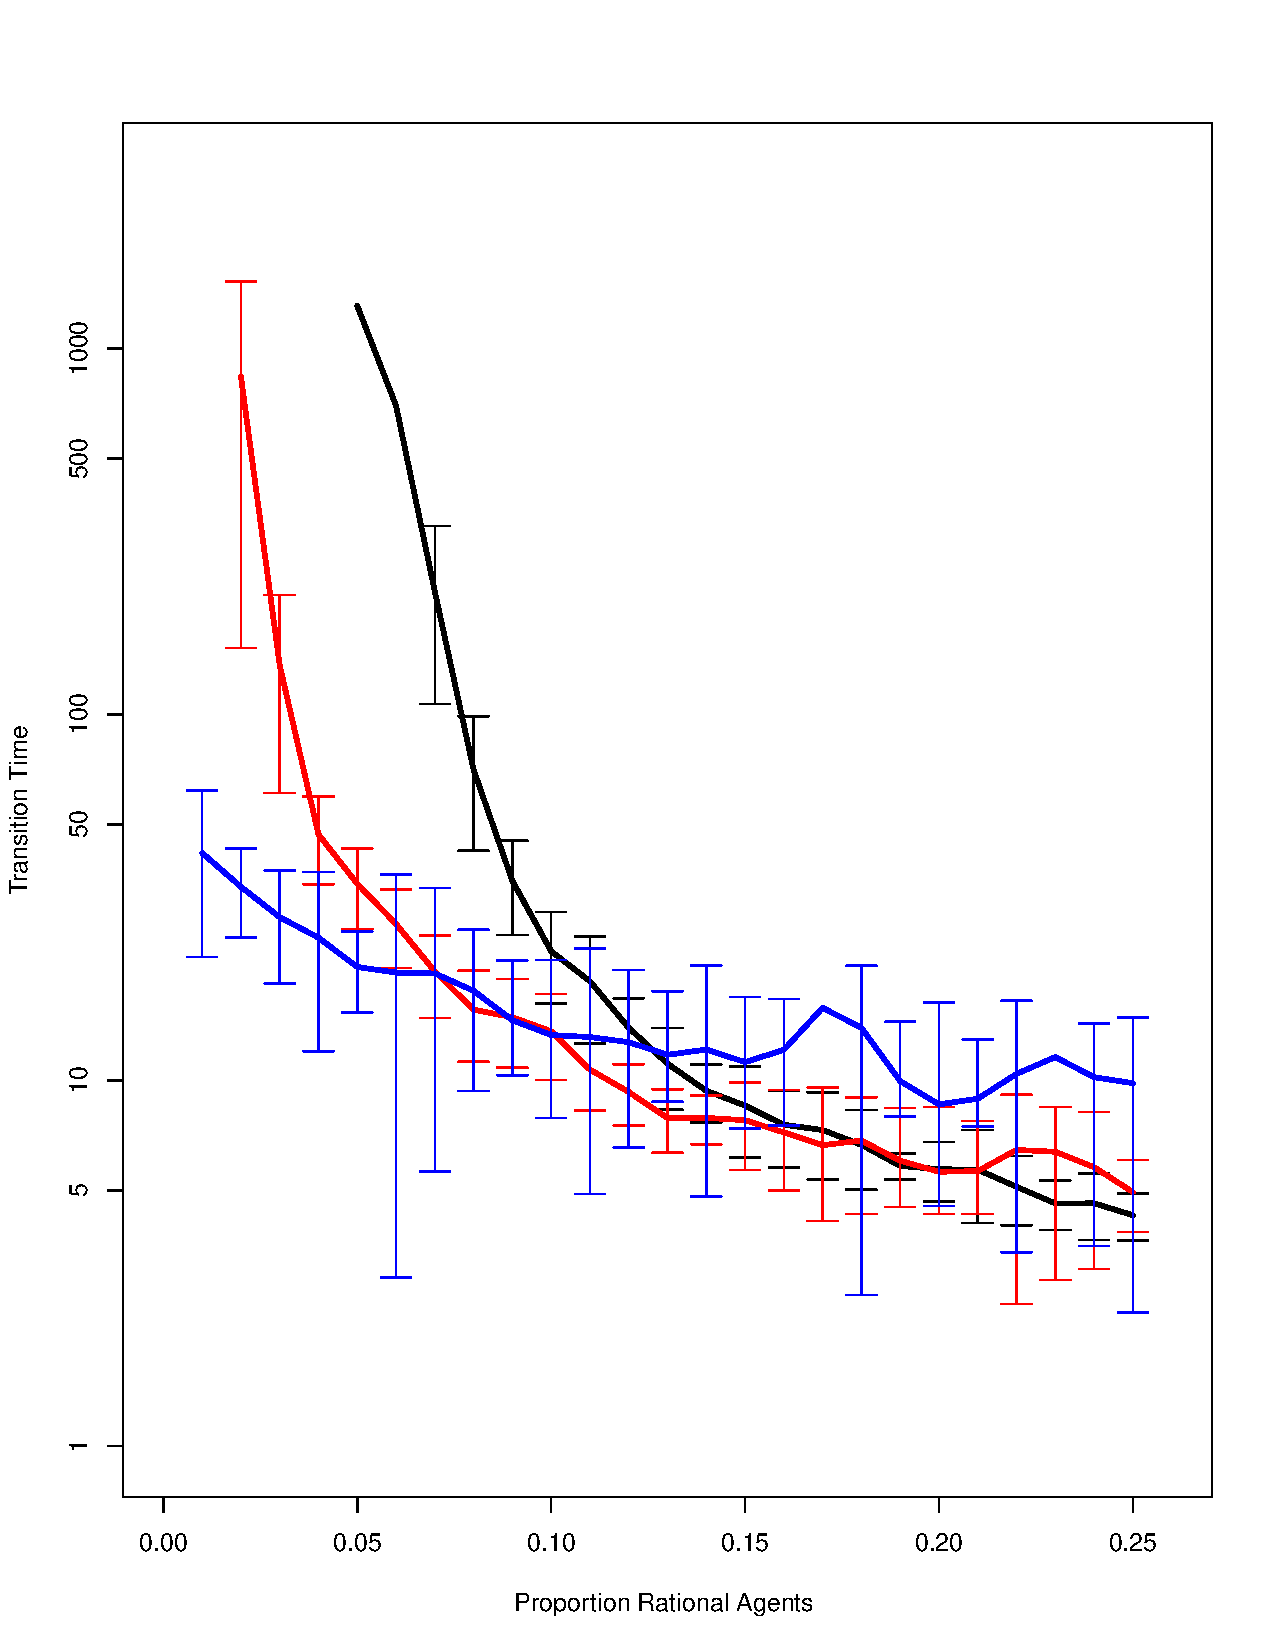
\includegraphics[scale =.25] {figs/figure6_replication.png}
 }

\caption{Rational agents sweep, black: 0\% random, red: 5\% random, blue 10\% random}
\label{figure6}
\end{figure}

We got better results when replicating changes in the maximum network size.
As figure~\ref{figure8} shows we replicate both the increase in average and standard deviation.
Again, we failed to achieve numerical identity.
Our model can be 10 times faster in reaching full-retirement state.

\begin{figure}
\centering
  \subfigure[Original Paper]{
   \includegraphics[scale =.70] {figs/figure8.png}
 }
 \subfigure[MASON replication]{
   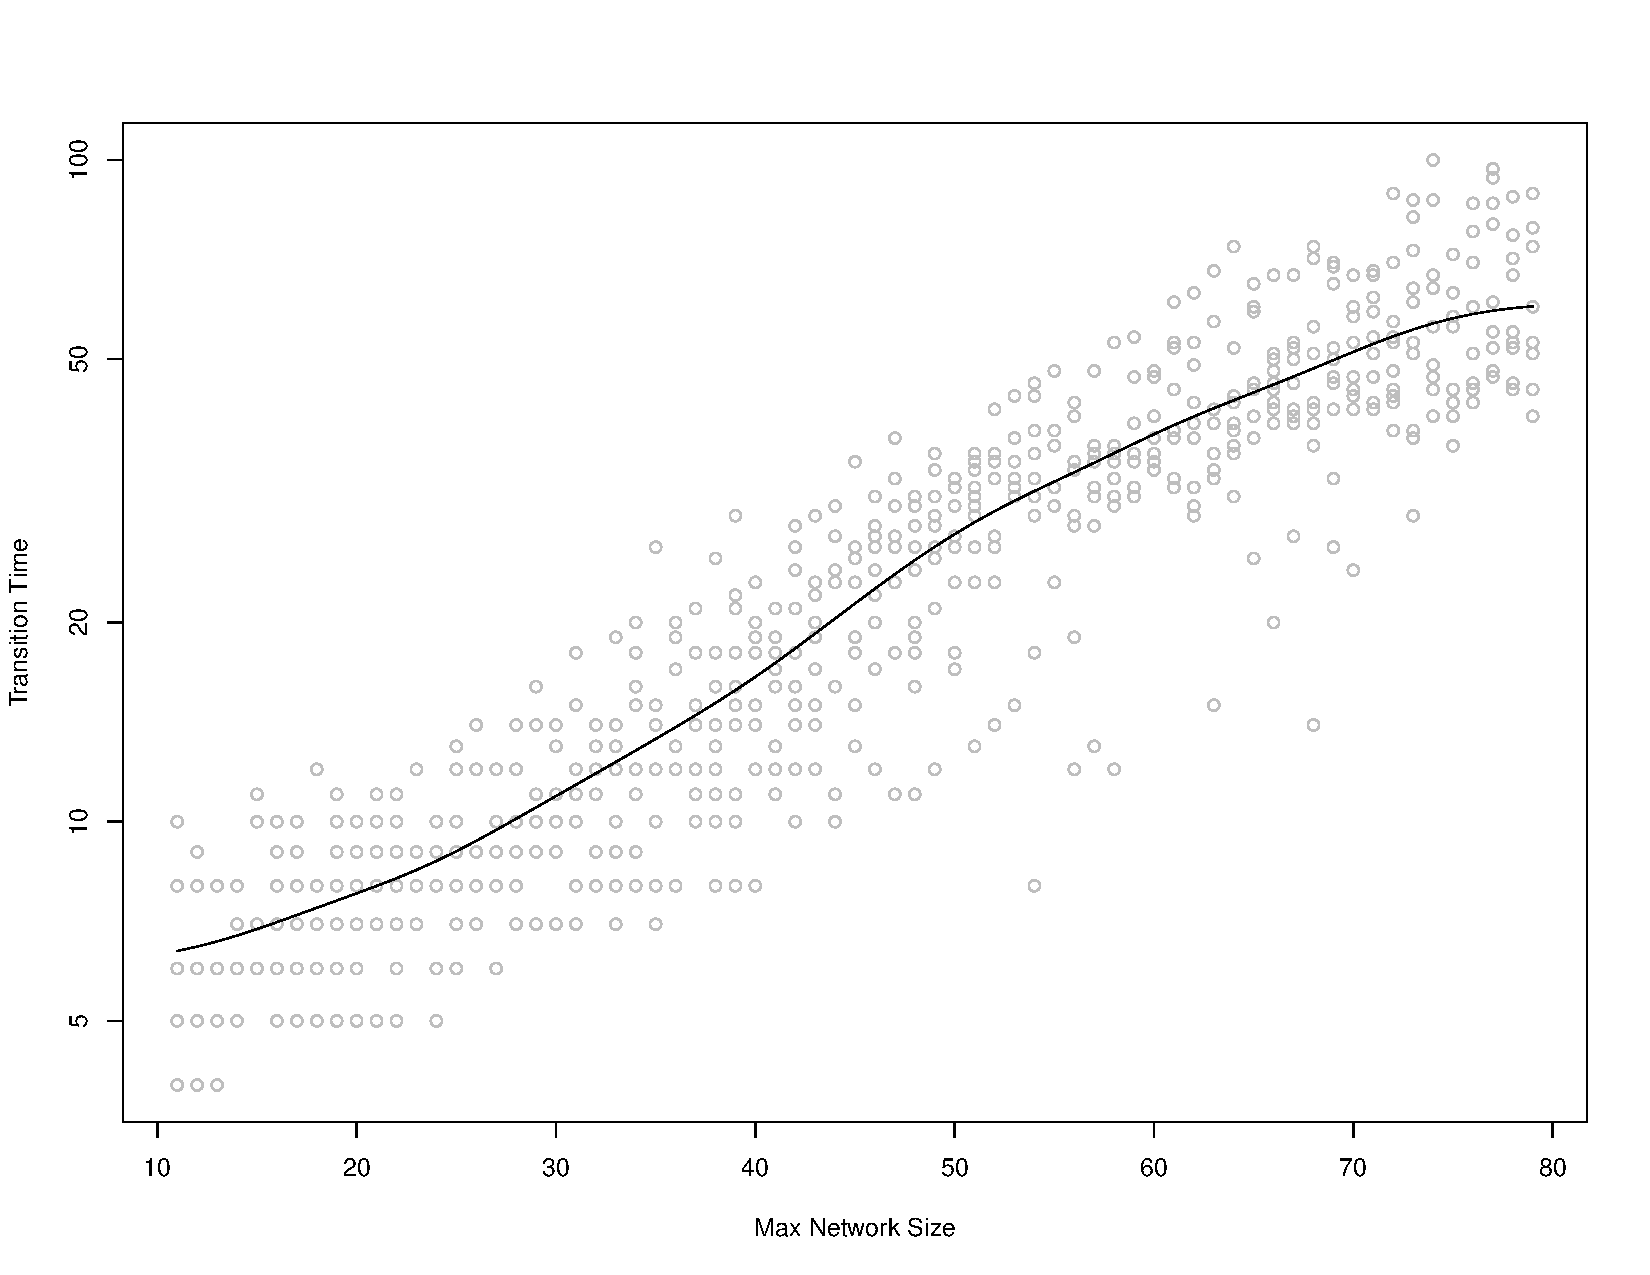
\includegraphics[scale =.25] {figs/figure8_replication.png}
 }

\caption{Changes in time to get full-retirement equilibrium by changing maximum network size. Grey dots represent runs}
\label{figure8}
\end{figure}

\subsection{Transition from 65 to 62}

The attempt to replicate retirement dynamics when age limit passes from 65 to 62 was a failure.
The original paper mimic real data: society moves slowly from one equilibrium to the next.
In particular it was shown that the higher the proportion of imitators the more slowly such result was obtained.

In our model transition dynamic are markedly non-linear.
Specifically, either the transition occur almost instantly or it never happens.
In fact, when the transition fails a new equilibrium with almost everyone working emerges.

Very interestingly is that we can get somewhat more similar results to the paper if we focus on transition from 65 to 60 instead.
In this case the transition is quick but not instantaneous and dependant on the population proportions.

It is instructive as it streches the definition of relational equivalence.
In this case, at first sight, it looks like a utter failure.
But with a slight modification of the target we can get more reasonable fits.

\subsection{Threshold dynamic}

We find that whether imitator agents follow their threshold strictly or not is very important.
When exactly half of the eligibles friends have retired, should the agent retire as well?
To show the effects we fix the number of rational agents to 10\% and we run the same simulation fixing the seed.
Figure~\ref{laxstrict} show the result of the simulation.

\begin{figure}
 \begin{center}
  \includegraphics[scale=.30]{figs/laxstrict.png}
\caption{The black line is the simulation with strict threshold, the red line is without}
\label{laxstrict}
 \end{center}
\end{figure}

This highlights one of the oft-neglected advantages of replication.
Whenever the original source code is missing, only through replication one is able to make additional tests on someone else's model.

This goes also to show that minor assumptions might have great impact.
In this case a change in threshold from $.5$ to $.499$ mean the difference between mass retirement and perennial work.

\section{Conclusion}

In this paper we tried to singlemindedly focus on replication.
We chose the retirement model because its dynamics are simple and its behavior rules easy to program.

In spite of this we could only partially replicate results.
This casts serious concerns over replication in general.
It underlines how access to the original source code is a must.

We also tested some of the advantages and disadvantages of programming with MASON.
This model was too simple to take advantage of many of the features of Java.
Nevertheless even for such elementary model object orientation proved helpful.
Unfortunately we also spent much time fixing garbage collection issues due to MASON and Java misuse.
Programming got in the way of modeling.






\bibliographystyle{splncs03}
\bibliography{references}

\end{document}
